%%=============================================================================
%% Proof of Concept
%%=============================================================================

\chapter{\IfLanguageName{dutch}{Proof of Concept}{Proof of Concept}}%
\label{ch:proof-of-concept}

Dit deel van het onderzoek presenteert een proof of concept gericht op de beoordeling van de gekozen navigatiemethoden die gebruikt kunnen worden voor mensen met een mentale beperking. Het doel van de proof of concept is de efficiëntie, bruikbaarheid en gebruiksvriendelijkheid van deze methoden te onderzoeken aan de hand van een applicatie. De ontwikkeling van deze applicatie en hieruit gehaalde resultaten worden besproken. Als laatste zal er besproken worden welke navigatietool de meest geschikte is voor de doelgroep.

\section{Ontwikkeling van de applicatie}
\label{sec:ontwikkeling van de applicatie}
In dit onderdeel wordt de opbouw van de applicatie besproken. Hieruit zal duidelijk worden hoe de applicatie opgebouwd is. De code is niet relevant voor het verdere verloop van het onderzoek. Als eerste worden de belangrijkste onderdelen besproken. Een nieuw React Native project wordt aangemaakt aan de hand van Node.js en een terminal. Na het opzetten van dit project, moet er een Mapbox account gecreëerd worden om een publieke token te kunnen verkrijgen zodat er gebruik gemaakt kan worden van hun diverse mappen. \newline

De applicatie bestaat uit één eenvoudig scherm. Op Figuur \ref{fig:Scherm met een knop om de route op te vragen} is te zien dat er een Mapbox map ingeladen wordt en een invoerveld met een knop. Het proces wordt in gang gezet wanneer op de knop gedrukt wordt en een correct adres is ingegeven. Wanneer een foutief adres wordt ingegeven zal er een foutmelding komen en wordt het proces onderbroken. Bij Figuur \ref{fig:Scherm met knop waar route die opgevraagd is} is de route gegeneerd die op het scherm komt wanneer op de knop gedrukt wordt en een correct adres ingegeven is.

%begin{lstlisting}[caption={Code-voorbeeld van het navigatiescherm}, label=code-voorbeeld navigatiescherm, captionpos=b]
%    Mapbox.setAccessToken('MAPBOX_PUBLIC_TOKEN');
%    
%    const App = () => {
%        const [location, setLocation] = useState('');
%        const [destination, setDestination] = useState('');
%        const [route, setRoute] = useState(null);
%        const [errorMsg, setErrorMsg] = useState(null);
%        const [isLoading, setIsLoading] = useState(false);
%        
%        useEffect(() => {
%            (async () => {
%                let { status } = await Location.requestForegroundPermissionsAsync();
%                if (status !== 'granted') {
%                    setErrorMsg('Permission to access location was denied');
%                    return;
%                }
%                
%                let currentLocation;
%                if (Platform.OS === 'OS' && !__DEV__) {
%                    currentLocation = await Location.getCurrentPositionAsync({});
%                    console.log('Current location:', currentLocation);
%                } else {
%                    currentLocation = {
%                        coords: {
%                            longitude: 4.038139399999999,
%                            latitude: 50.9318886,
%                        },
%                    };
%                }
%                
%                if (!currentLocation) {
%                    setErrorMsg('Failed to obtain location');
%                    return;
%                }
%                setLocation(currentLocation);
%            })();
%        }, []);
%        
%        const getRoute = async () => {
%            setIsLoading(true);
%            const userLocation = `${location.coords.longitude},${location.coords.latitude}`;
%            console.log('User location:', userLocation);
%            
%            const YOUR_GOOGLE_API_KEY = 'GOOGLE_API_KEY';
%            
%            const startLong = location.coords.longitude;
%            const startLat = location.coords.latitude;
%            
%            try {
%                const destinationCoords = await getCoordinatesFromPlace(destination, YOUR_GOOGLE_API_KEY);
%                const endLong = destinationCoords.split(',')[1];
%                const endLat = destinationCoords.split(',')[0];
%                console.log(endLong, endLat)
%                console.log('Destination coordinates:', destinationCoords);
%                if(!destinationCoords) {
%                    throw new Error('Failed to fetch destination coordinates');
%                }
%                
%                const mapboxUrl = `https://api.mapbox.com/directions/v5/mapbox/walking/${startLong},${startLat};${endLong},${endLat}?alternatives=true&annotations=distance&continue_straight=true&geometries=geojson&overview=full&steps=false&access_token=MAPBOX_PUBLIC_TOKEN`
%                console.log('Mapbox Directions API URL:', mapboxUrl);
%                const response = await fetch(mapboxUrl);
%                const data = await response.json();
%                                
%                if (data.routes && data.routes.length > 0) {
%                    const routeCoordinates = data.routes[0].geometry.coordinates.map(coord => ({ longitude: coord[0], latitude: coord[1] }));
%                    // console.log('Route coordinates:', routeCoordinates);
%                    setRoute(routeCoordinates);
%                } else if (data.coords == 'NoRoute'){
%                    throw new Error('No route found');
%                } else {
%                    throw new Error('Failed to fetch route');
%                }
%            } catch (error) {
%                console.error(error);
%                setErrorMsg('Failed to fetch route');
%            } finally {
%                setIsLoading(false);
%            }
%        };
%        
%        const getCoordinatesFromPlace = async (place, apiKey) => {
%            const apiUrl = `https://maps.googleapis.com/maps/api/geocode/json?address=${encodeURIComponent(place)}&key=${apiKey}`;
%            
%            try {
%                const response = await fetch(apiUrl);
%                
%                console.log('Geocoding API response status:', response.status);
%                
%                if (!response.ok) {
%                    throw new Error(`Geocoding API request failed with status ${response.status}`);
%                }
%                
%                const data = await response.json();
%                                
%                if (data.status === 'OK' && data.results.length > 0) {
%                    const result = data.results.find(result => result && result.geometry && result.geometry.location);
%                    if (result) {
%                        const { lat, lng } = result.geometry.location;
%                        console.log('Geocoding result:', lat, lng);
%                        return `${lat},${lng}`;
%                    } else {
%                        throw new Error('No valid location found in the geocoding results');
%                    }
%                } else {
%                    throw new Error(`Geocoding failed: ${data.status || 'Unknown error'}`);
%                }
%            } catch (error) {
%                console.error('Error in getCoordinatesFromPlace:', error);
%                throw error;
%            }
%        };
%        
%        const renderRouteLine = () => {
%            if (!route) {
%                return null; 
%            }
%            
%            const routeCoordinates = route.map(coord => [coord.longitude, coord.latitude]);
%            // console.log("Route coordinates:", route);
%            return (
%            <Mapbox.ShapeSource id="routeSource" shape={{
%                    type: 'Feature',
%                    geometry: {
%                        type: 'LineString',
%                        coordinates: routeCoordinates,
%                    },
%            }}>
%            <Mapbox.LineLayer id="routeFill" style={{ lineColor: 'blue', lineWidth: 3 }} />
%            </Mapbox.ShapeSource>
%            );
%        };
%        
%        if (!location || !location.coords) {
%            return (
%            <View style={styles.container}>
%            <ActivityIndicator size="large" />
%            <Text>{errorMsg || 'Waiting for location...'}</Text>
%            </View>
%            );
%        }
%        
%        return (
%        <View style={styles.container}>
%        <Mapbox.MapView style={styles.map}>
%        <Mapbox.Camera
%        zoomLevel={13}
%        centerCoordinate={[location.coords.longitude, location.coords.latitude]}
%        />
%        <Mapbox.UserLocation />
%        {route && renderRouteLine()}
%        </Mapbox.MapView>
%        
%        {/* Destination Input Field */}
%        <View style={styles.inputContainer}>
%        <TextInput
%        style={styles.input}
%        placeholder="Enter destination address"
%        value={destination}
%        onChangeText={setDestination}
%        />
%        <Button title="Get Route" onPress={getRoute} disabled={isLoading} />
%        </View>
%        
%        {isLoading && (
%            <View style={styles.loading}>
%            <ActivityIndicator size="large" />
%            </View>
%            )}
%        </View>
%        );
%    };
%    
%    export default App;
%    
%    const styles = StyleSheet.create({
%        container: {
%            ...StyleSheet.absoluteFillObject,
%            justifyContent: 'flex-end',
%            alignItems: 'center',
%        },
%        map: {
%            ...StyleSheet.absoluteFillObject,
%        },
%        inputContainer: {
%            width: '100%',
%            marginBottom: 20,
%        },
%        input: {
%            width: '90%',
%            paddingHorizontal: 10,
%            borderWidth: 1,
%            borderColor: '#ccc',
%            borderRadius: 5,
%            height: 40,
%            backgroundColor: '#fff',
%            marginBottom: 10,
%        },
%        loading: {
%            position: 'absolute',
%            top: '50%',
%            left: '50%',
%            zIndex: 1,
%            transform: [{ translateX: -25 }, { translateY: -25 }],
%        },
%    });
%\end{lstlisting}


\begin{figure}[htbp]
    \centering
    \begin{minipage}[b]{0.45\textwidth}
        \centering
        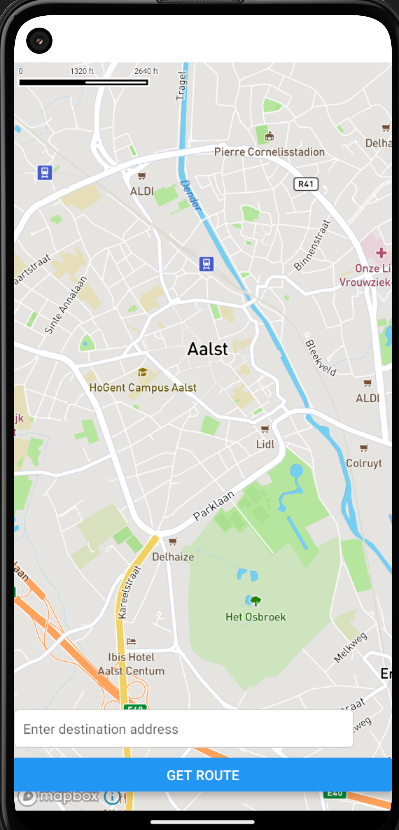
\includegraphics[width=\textwidth]{image.png}
        \caption{Scherm met een knop om de route op te vragen}
        \label{fig:Scherm met een knop om de route op te vragen}
    \end{minipage}
    \hspace{0.05\textwidth}
    \begin{minipage}[b]{0.45\textwidth}
        \centering
        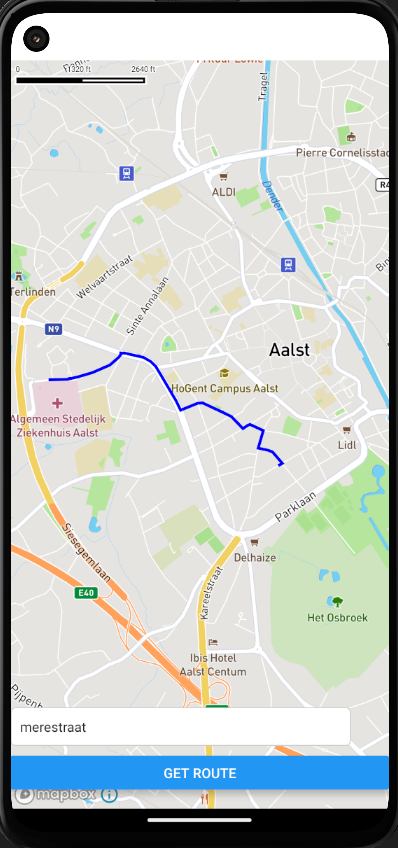
\includegraphics[width=\textwidth]{image-1.png}
        \caption{Scherm met knop waar de route die opgevraagd is}
        \label{fig:Scherm met knop waar route die opgevraagd is}
    \end{minipage}
\end{figure}

\subsection{Installatie en opstarten van de applicatie}
\label{sec:installatie en opstarten van de applicatie}

Zorg ervoor dat Node.js geïnstalleerd is op je systeem en in je \texttt{\$PATH} variabelen staat.
een Mapbox publieke token is nodig om de kaarten te kunnen gebruiken.

\begin{enumerate}
    \item Clone de repository.
    \item Voer `npm install` uit in de hoofdmap van de repository.
    \item In \texttt{App.js}, vervang 'YOUR\_MAPBOX\_PUBLIC\_KEY' door je eigen Mapbox publieke token.
    \item Bij \textbf{MapboxUrl} in \texttt{App.js}, vervang \texttt{key=YOUR\_MAPBOX\_PUBLIC\_KEY} aan het einde van de URL met je eigen Mapbox publieke token.
    \item Je hebt ook een \textbf{Google API key} \texttt{YOUR\_GOOGLE\_API\_KEY} nodig voor het maken van de route. Deze kan je verkrijgen op de Google Cloud Platform\footnote{\url{https://cloud.google.com/?hl=nl}}.
    \item Voer `npx expo start` uit om de applicatie te starten. Je kan de optie \texttt{--android} of \texttt{--ios} toevoegen om de applicatie te starten in een specifieke emulator.
    \item Selecteer een emulator of scan de QR code met de Expo app op je telefoon.
\end{enumerate}


\section{Mapbox}
\label{sec:mapbox}

\subsection*{Algemene bruikbaarheid}
Mapbox biedt een veelzijdig platform voor het maken van op maat gemaakte kaarten en locatiegebaseerde applicaties. Het wordt voor hoge aanpasbaarheid, nauwkeurige kaarten en robuuste API's gebruikt. Het platform is geschikt voor verschillende gebruiksscenario's, van eenvoudige kaartintegraties tot complexe data-analyse en visualisaties.

\subsection*{Platform}
Mapbox ondersteunt meerdere platformen, waaronder web, iOS en Android. Het biedt SDK's en API's die integratie met populaire frameworks en programmeertalen zoals JavaScript, Swift en Kotlin mogelijk maken. Hierdoor is Mapbox een flexibele keuze voor ontwikkelaars die kaarten in hun applicaties willen integreren.

\subsection*{Intuïtiviteit}
De gebruikersinterface van Mapbox Studio is ontworpen voor zowel beginners als gevorderde gebruikers. Het biedt een grafische interface voor het ontwerpen en aanpassen van kaarten zonder dat er uitgebreide programmeerkennis vereist is. Voor meer geavanceerde gebruikers is er uitgebreide documentatie beschikbaar.

\subsection*{Platformonafhankelijkheid}
Mapbox is platformonafhankelijk en kan worden gebruikt in verschillende omgevingen, waaronder mobiele apparaten, desktops en het web. Dit maakt het een veelzijdige oplossing voor diverse aan toestellen.

\subsection*{Visuele aanwijzingen}
Mapbox biedt uitgebreide mogelijkheden voor het toevoegen van visuele aanwijzingen, zoals aangepaste markeringen, AR-toepassingen, $\ldots$. Dit helpt gebruikers om gemakkelijk hun weg te vinden.

\subsection*{Auditieve instructies}
Hoewel Mapbox zelf geen ingebouwde auditieve instructies biedt, kan het worden geïntegreerd met andere diensten en tools die spraaknavigatie ondersteunen. Ontwikkelaars kunnen bijvoorbeeld gebruikmaken van Text-to-Speech (TTS) APIs om auditieve aanwijzingen te genereren.

\subsection*{Real-time updates}
Mapbox ondersteunt real-time updates, waardoor kaarten dynamisch kunnen worden bijgewerkt met live data. Dit is essentieel voor toepassingen zoals verkeersinformatie of andere situaties waarbij actuele informatie cruciaal is.

\subsection*{Toegankelijkheidsfuncties}
Mapbox biedt diverse toegankelijkheidsfuncties, zoals ondersteuning voor screen readers en mogelijkheden voor het aanpassen van kleuren en contrasten om kaarten toegankelijker te maken voor een bredere doelgroep. 

\subsection*{Connectiviteit}
Mapbox vereist internetconnectiviteit voor het laden van kaarten en het ophalen van real-time data. Echter, het biedt ook mogelijkheden voor offline gebruik door kaarten vooraf te downloaden en lokaal op te slaan.

\subsection*{Aanpasbaarheid}
Een van de sterke punten van Mapbox is de hoge mate van aanpasbaarheid. Gebruikers kunnen vrijwel elk aspect van hun kaarten aanpassen, inclusief stijl, gegevensbronnen, en interactieve elementen. Dit maakt het mogelijk om kaarten te creëren die precies voldoen aan de specifieke behoeften van een project.

\subsection*{Offline functionaliteit}
Mapbox ondersteunt offline functionaliteit door het mogelijk te maken om kaarttegels en andere gegevens vooraf te downloaden en lokaal op te slaan. Dit is bijzonder nuttig voor toepassingen in gebieden met beperkte of geen internettoegang.

\subsection*{Veiligheidsfuncties}
Mapbox biedt verschillende veiligheidsfuncties, zoals versleuteling van dataoverdracht en authenticatie via API-sleutels. Dit helpt om de integriteit en veiligheid van de gegevens en de applicaties te waarborgen.

\subsection*{Visual noise}
Mapbox biedt tools om visuele ruis te minimaliseren door gebruikers de mogelijkheid te geven om overbodige details te verwijderen en de kaartweergave te optimaliseren voor duidelijkheid en gebruiksgemak. Dit is essentieel om de kaart leesbaar en nuttig te houden.

\subsection*{Speciale hardware}
Mapbox vereist geen speciale hardware en kan worden gebruikt op standaard computers en mobiele apparaten. Dit maakt het toegankelijk voor een groot aantal aan gebruikers en toepassingen.

\subsection*{Het navigatieproces moet snel zijn, om tijdverlies en onzekerheid te minimaliseren}
Mapbox is geoptimaliseerd voor snelle laadtijden en eenvoudige navigatie. De prestaties van de kaarten zijn geoptimaliseerd om snel te reageren op gebruikersinvoer en real-time data-integratie te ondersteunen, wat cruciaal is voor een efficiënte navigatie-ervaring.

\subsection*{De informatie die de gebruiker moet onthouden moet beperkt zijn, om het risico op fouten te verlagen}
Mapbox stelt gebruikers in staat om kaarten zo te ontwerpen dat ze alleen de essentiële informatie tonen, waardoor cognitieve belasting wordt verminderd en de kans op fouten afneemt. Dit wordt bereikt door de mogelijkheid om lagen en gegevens te filteren en te configureren naar eigen voorkeur.

\subsection*{Het aantal stappen in het navigatieproces moet tot een minimum beperkt blijven}
Met Mapbox kunnen ontwikkelaars intuïtieve en directe navigatieoplossingen creëren die het aantal benodigde stappen minimaliseren. Functies zoals duidelijke routebeschrijvingen en interactieve elementen dragen bij aan een gestroomlijnde gebruikerservaring.

\subsection*{De navigatiemethodes moeten gebruiksvriendelijk zijn voor mensen met dyslexie. Er moet rekening gehouden worden met de lees- en onthoudmoeilijkheden die zij kunnen ervaren}
Mapbox maakt het mogelijk om de vormgeving van kaarten en tekst aan te passen om de leesbaarheid te verbeteren voor mensen met dyslexie. Dit kan onder andere door het gebruik van geschikte lettertypen, kleuren en contrasten. Ook met behulp van AI kunnen voorstellen van locaties gedaan worden.

\subsection*{Het zou voordelig zijn als de navigatiemethodes kostenefficiënt zijn, zodat onnodige kosten vermeden worden, wat de dienst toegankelijker maakt voor de eindgebruiker en de aanbieder}
Mapbox biedt flexibele prijsmodellen, waaronder een gratis tier voor basisgebruik en schaalbare betalingsopties voor geavanceerdere toepassingen. Dit maakt het mogelijk om kostenefficiënte navigatieoplossingen te implementeren die aansluiten bij de behoeften en budgetten van verschillende gebruikers.

\section{Google Maps}
\label{sec:google maps}

\subsection*{Algemene bruikbaarheid}
Google Maps biedt gedetailleerde routebeschrijvingen, verkeersinformatie, en zoekfuncties voor nabijgelegen locaties.

\subsection*{Platform}
Google Maps is beschikbaar op meerdere platformen, waaronder web, iOS en Android. Het biedt een sterke integratie met andere Google-diensten en heeft een uitgebreide API voor ontwikkelaars om kaarten en locatiegebaseerde functies in hun eigen applicaties te integreren.

\subsection*{Intuïtiviteit}
De intuïtiviteit van Google Maps is hoog, met een eenvoudige en overzichtelijke interface. Gebruikers kunnen gemakkelijk zoeken naar locaties, routes plannen en informatie over verkeersomstandigheden en openbaar vervoer bekijken. De applicatie maakt gebruik van de bekende Google UI/UX patronen.

\subsection*{Platformonafhankelijkheid}
De applicatie werkt naadloos op verschillende platformen en apparaten, inclusief desktops, laptops, tablets en smartphones. De gebruikerservaring is consistent en optimaal ongeacht het gebruikte apparaat.

\subsection*{Visuele aanwijzingen}
Google Maps biedt uitgebreide visuele aanwijzingen, waaronder gedetailleerde kaarten, satellietbeelden, street view, live view of AR en 3D-kaarten. Gebruikers kunnen eenvoudig locaties herkennen en routes volgen dankzij de visuele ondersteuning.

\subsection*{Auditieve instructies}
De applicatie biedt spraakgestuurde navigatie met duidelijke auditieve instructies. Dit is vooral handig tijdens het rijden of wandelen, omdat gebruikers niet naar hun mobielscherm hoeven te kijken om te weten welke richting ze op moeten.

\subsection*{Real-time updates}
Google Maps biedt real-time updates voor verkeersinformatie, openbaar vervoer, en veranderingen in routes. Dit zorgt ervoor dat gebruikers altijd de meest actuele informatie hebben tijdens hun reis, wat helpt bij het vermijden van vertragingen en files.

\subsection*{Toegankelijkheidsfuncties}
De applicatie heeft verschillende toegankelijkheidsfuncties, zoals ondersteuning voor screen readers, gesproken aanwijzingen en opties voor aangepaste weergave-instellingen om de leesbaarheid te verbeteren.

\subsection*{Connectiviteit}
Google Maps vereist internetconnectiviteit voor de meeste functies, zoals het ophalen van kaarten, real-time verkeersinformatie en routebeschrijvingen. Er zijn echter ook offline kaarten beschikbaar die gebruikers kunnen downloaden voor gebruik zonder internetverbinding.

\subsection*{Aanpasbaarheid}
Google Maps is niet zo aanpasbaar is als Mapbox. Het biedt wel enkele aanpassingsopties via de Google Maps API. Ontwikkelaars kunnen kaarten integreren en aanpassen binnen hun eigen applicaties, hoewel de mogelijkheden voor aanpassing beperkt zijn in vergelijking met meer specifieke oplossingen.

\subsection*{Offline functionaliteit}
De applicatie biedt offline functionaliteit door gebruikers toe te staan kaarten van specifieke gebieden te downloaden en op te slaan op hun apparaat. Dit is handig voor het verplaatsen in gebieden met weinig of geen internettoegang.

\subsection*{Veiligheidsfuncties}
Google Maps zorgt voor de veiligheid van gegevens door gebruik te maken van versleuteling en veilige verbindingen. Bovendien biedt het functies zoals locatie delen, waarmee gebruikers hun live locatie kunnen delen met vertrouwde contacten tijdens het navigeren of verplaatsen.

\subsection*{Visual noise}
Google Maps minimaliseert visuele ruis door een schone en overzichtelijke kaartweergave te bieden. Gebruikers kunnen ongewenste lagen en informatie uitschakelen om de weergave aan te passen aan hun behoeften.

\subsection*{Speciale hardware}
De applicatie vereist geen speciale hardware en werkt op standaard apparaten zoals smartphones, tablets en computers. Dit maakt het breed toegankelijk voor verschillende gebruikers.

\subsection*{Het navigatieproces moet snel zijn, om tijdverlies en onzekerheid te minimaliseren}
Google Maps is geoptimaliseerd voor snelle en efficiënte navigatie. Het biedt direct routebeschrijvingen en alternatieve routes om tijdverlies en onzekerheid te minimaliseren. Real-time verkeersinformatie helpt bij het optimaliseren van de tijd die nodig is om zich te verplaatsen.

\subsection*{De informatie die de gebruiker moet onthouden moet beperkt zijn, om het risico op fouten te verlagen}
Google Maps presenteert informatie op een duidelijke en beknopte manier, waardoor de hoeveelheid informatie die de gebruiker moet onthouden wordt geminimaliseerd. Spraakgestuurde aanwijzingen en visuele markeringen helpen gebruikers om gemakkelijk hun weg te vinden zonder veel details te moeten onthouden.

\subsection*{Het aantal stappen in het navigatieproces moet tot een minimum beperkt blijven}
De applicatie biedt een gestroomlijnd navigatieproces met minimale stappen. Gebruikers kunnen snel een bestemming invoeren, een route selecteren en beginnen met navigeren. De interface is ontworpen om het aantal benodigde acties te minimaliseren.

\subsection*{De navigatiemethodes moeten gebruiksvriendelijk zijn voor mensen met dyslexie. Er moet rekening gehouden worden met de lees- en onthoudmoeilijkheden die zij kunnen ervaren}
Google Maps houdt rekening met toegankelijkheid en biedt verschillende functies om de gebruiksvriendelijkheid voor mensen met dyslexie te verbeteren, zoals duidelijke en beknopte tekstweergave, ondersteuning voor spraakgestuurde zoekopdrachten en aanwijzingen. De applicatie doet ook voorstellen in van locaties die ingevoerd worden.

\subsection*{Het zou voordelig zijn als de navigatiemethodes kostenefficiënt zijn, zodat onnodige kosten vermeden worden, wat de dienst toegankelijker maakt voor de eindgebruiker en de aanbieder}
Google Maps is gratis te gebruiken, wat het een kostenefficiënte optie maakt voor navigatie. Voor bedrijven en ontwikkelaars biedt Google Maps Platform betaalde plannen.

\section{Samenvatting}
\label{sec:samenvatting}







